\documentclass[twoside]{book}

% Packages required by doxygen
\usepackage{calc}
\usepackage{doxygen}
\usepackage{graphicx}
\usepackage[utf8]{inputenc}
\usepackage{makeidx}
\usepackage{multicol}
\usepackage{multirow}
\usepackage{textcomp}
\usepackage[table]{xcolor}

% Font selection
\usepackage[T1]{fontenc}
\usepackage{mathptmx}
\usepackage[scaled=.90]{helvet}
\usepackage{courier}
\usepackage{amssymb}
\usepackage{sectsty}
\renewcommand{\familydefault}{\sfdefault}
\allsectionsfont{%
  \fontseries{bc}\selectfont%
  \color{darkgray}%
}
\renewcommand{\DoxyLabelFont}{%
  \fontseries{bc}\selectfont%
  \color{darkgray}%
}

% Page & text layout
\usepackage{geometry}
\geometry{%
  a4paper,%
  top=2.5cm,%
  bottom=2.5cm,%
  left=2.5cm,%
  right=2.5cm%
}
\tolerance=750
\hfuzz=15pt
\hbadness=750
\setlength{\emergencystretch}{15pt}
\setlength{\parindent}{0cm}
\setlength{\parskip}{0.2cm}
\makeatletter
\renewcommand{\paragraph}{%
  \@startsection{paragraph}{4}{0ex}{-1.0ex}{1.0ex}{%
    \normalfont\normalsize\bfseries\SS@parafont%
  }%
}
\renewcommand{\subparagraph}{%
  \@startsection{subparagraph}{5}{0ex}{-1.0ex}{1.0ex}{%
    \normalfont\normalsize\bfseries\SS@subparafont%
  }%
}
\makeatother

% Headers & footers
\usepackage{fancyhdr}
\pagestyle{fancyplain}
\fancyhead[LE]{\fancyplain{}{\bfseries\thepage}}
\fancyhead[CE]{\fancyplain{}{}}
\fancyhead[RE]{\fancyplain{}{\bfseries\leftmark}}
\fancyhead[LO]{\fancyplain{}{\bfseries\rightmark}}
\fancyhead[CO]{\fancyplain{}{}}
\fancyhead[RO]{\fancyplain{}{\bfseries\thepage}}
\fancyfoot[LE]{\fancyplain{}{}}
\fancyfoot[CE]{\fancyplain{}{}}
\fancyfoot[RE]{\fancyplain{}{\bfseries\scriptsize Generated on Fri May 9 2014 20\-:34\-:26 for o\-Mush by Doxygen }}
\fancyfoot[LO]{\fancyplain{}{\bfseries\scriptsize Generated on Fri May 9 2014 20\-:34\-:26 for o\-Mush by Doxygen }}
\fancyfoot[CO]{\fancyplain{}{}}
\fancyfoot[RO]{\fancyplain{}{}}
\renewcommand{\footrulewidth}{0.4pt}
\renewcommand{\chaptermark}[1]{%
  \markboth{#1}{}%
}
\renewcommand{\sectionmark}[1]{%
  \markright{\thesection\ #1}%
}

% Indices & bibliography
\usepackage{natbib}
\usepackage[titles]{tocloft}
\setcounter{tocdepth}{3}
\setcounter{secnumdepth}{5}
\makeindex

% Hyperlinks (required, but should be loaded last)
\usepackage{ifpdf}
\ifpdf
  \usepackage[pdftex,pagebackref=true]{hyperref}
\else
  \usepackage[ps2pdf,pagebackref=true]{hyperref}
\fi
\hypersetup{%
  colorlinks=true,%
  linkcolor=blue,%
  citecolor=blue,%
  unicode%
}

% Custom commands
\newcommand{\clearemptydoublepage}{%
  \newpage{\pagestyle{empty}\cleardoublepage}%
}


%===== C O N T E N T S =====

\begin{document}

% Titlepage & ToC
\hypersetup{pageanchor=false}
\pagenumbering{roman}
\begin{titlepage}
\vspace*{7cm}
\begin{center}%
{\Large o\-Mush }\\
\vspace*{1cm}
{\large Generated by Doxygen 1.8.6}\\
\vspace*{0.5cm}
{\small Fri May 9 2014 20:34:26}\\
\end{center}
\end{titlepage}
\clearemptydoublepage
\tableofcontents
\clearemptydoublepage
\pagenumbering{arabic}
\hypersetup{pageanchor=true}

%--- Begin generated contents ---
\chapter{Namespace Index}
\section{Namespace List}
Here is a list of all documented namespaces with brief descriptions\-:\begin{DoxyCompactList}
\item\contentsline{section}{\hyperlink{namespaceomush}{omush} }{\pageref{namespaceomush}}{}
\end{DoxyCompactList}

\chapter{Hierarchical Index}
\section{Class Hierarchy}
This inheritance list is sorted roughly, but not completely, alphabetically\-:\begin{DoxyCompactList}
\item \contentsline{section}{omush\-:\-:Signal\-Handler}{\pageref{classomush_1_1_signal_handler}}{}
\item \contentsline{section}{omush\-:\-:Signal\-Handler\-Delegate}{\pageref{classomush_1_1_signal_handler_delegate}}{}
\begin{DoxyCompactList}
\item \contentsline{section}{omush\-:\-:Game}{\pageref{classomush_1_1_game}}{}
\end{DoxyCompactList}
\end{DoxyCompactList}

\chapter{Class Index}
\section{Class List}
Here are the classes, structs, unions and interfaces with brief descriptions\-:\begin{DoxyCompactList}
\item\contentsline{section}{\hyperlink{classomush_1_1command_1_1_command}{omush\-::command\-::\-Command} }{\pageref{classomush_1_1command_1_1_command}}{}
\item\contentsline{section}{\hyperlink{structomush_1_1command_1_1_command_factory}{omush\-::command\-::\-Command\-Factory} }{\pageref{structomush_1_1command_1_1_command_factory}}{}
\item\contentsline{section}{\hyperlink{classomush_1_1command_1_1_command_parser}{omush\-::command\-::\-Command\-Parser} }{\pageref{classomush_1_1command_1_1_command_parser}}{}
\item\contentsline{section}{\hyperlink{classomush_1_1command_1_1_command_quit}{omush\-::command\-::\-Command\-Quit} }{\pageref{classomush_1_1command_1_1_command_quit}}{}
\item\contentsline{section}{\hyperlink{structomush_1_1command_1_1_command_register}{omush\-::command\-::\-Command\-Register$<$ T $>$} }{\pageref{structomush_1_1command_1_1_command_register}}{}
\item\contentsline{section}{\hyperlink{classomush_1_1command_1_1_command_who}{omush\-::command\-::\-Command\-Who} }{\pageref{classomush_1_1command_1_1_command_who}}{}
\item\contentsline{section}{\hyperlink{classomush_1_1_database}{omush\-::\-Database} }{\pageref{classomush_1_1_database}}{}
\item\contentsline{section}{\hyperlink{classomush_1_1_database_object}{omush\-::\-Database\-Object} }{\pageref{classomush_1_1_database_object}}{}
\item\contentsline{section}{\hyperlink{classomush_1_1network_1_1_descriptor}{omush\-::network\-::\-Descriptor} }{\pageref{classomush_1_1network_1_1_descriptor}}{}
\item\contentsline{section}{\hyperlink{structomush_1_1_environment}{omush\-::\-Environment} }{\pageref{structomush_1_1_environment}}{}
\item\contentsline{section}{\hyperlink{classomush_1_1_exit}{omush\-::\-Exit} }{\pageref{classomush_1_1_exit}}{}
\item\contentsline{section}{\hyperlink{classomush_1_1_game}{omush\-::\-Game} }{\pageref{classomush_1_1_game}}{}
\item\contentsline{section}{\hyperlink{classomush_1_1network_1_1_input_queue}{omush\-::network\-::\-Input\-Queue} }{\pageref{classomush_1_1network_1_1_input_queue}}{}
\item\contentsline{section}{\hyperlink{classomush_1_1network_1_1_network}{omush\-::network\-::\-Network} }{\pageref{classomush_1_1network_1_1_network}}{}
\item\contentsline{section}{\hyperlink{classomush_1_1network_1_1_network_queue}{omush\-::network\-::\-Network\-Queue} }{\pageref{classomush_1_1network_1_1_network_queue}}{}
\item\contentsline{section}{\hyperlink{classomush_1_1network_1_1_output_queue}{omush\-::network\-::\-Output\-Queue} }{\pageref{classomush_1_1network_1_1_output_queue}}{}
\item\contentsline{section}{\hyperlink{classomush_1_1_player}{omush\-::\-Player} }{\pageref{classomush_1_1_player}}{}
\item\contentsline{section}{\hyperlink{classomush_1_1_room}{omush\-::\-Room} }{\pageref{classomush_1_1_room}}{}
\item\contentsline{section}{\hyperlink{classomush_1_1_signal_handler}{omush\-::\-Signal\-Handler} }{\pageref{classomush_1_1_signal_handler}}{}
\item\contentsline{section}{\hyperlink{classomush_1_1_signal_handler_delegate}{omush\-::\-Signal\-Handler\-Delegate} }{\pageref{classomush_1_1_signal_handler_delegate}}{}
\item\contentsline{section}{\hyperlink{classomush_1_1_thing}{omush\-::\-Thing} }{\pageref{classomush_1_1_thing}}{}
\end{DoxyCompactList}

\chapter{Namespace Documentation}
\hypertarget{namespaceomush}{\section{omush Namespace Reference}
\label{namespaceomush}\index{omush@{omush}}
}


Copyright 2014 Michael Smith.  


\subsection*{Classes}
\begin{DoxyCompactItemize}
\item 
class \hyperlink{classomush_1_1_database_object}{Database\-Object}
\item 
class \hyperlink{classomush_1_1_player}{Player}
\item 
class \hyperlink{classomush_1_1_thing}{Thing}
\item 
class \hyperlink{classomush_1_1_exit}{Exit}
\item 
class \hyperlink{classomush_1_1_room}{Room}
\item 
class \hyperlink{classomush_1_1_database}{Database}
\item 
struct \hyperlink{structomush_1_1_environment}{Environment}
\item 
class \hyperlink{classomush_1_1_game}{Game}
\item 
class \hyperlink{classomush_1_1_signal_handler_delegate}{Signal\-Handler\-Delegate}
\item 
class \hyperlink{classomush_1_1_signal_handler}{Signal\-Handler}
\end{DoxyCompactItemize}
\subsection*{Typedefs}
\begin{DoxyCompactItemize}
\item 
\hypertarget{namespaceomush_a4f95cdc9f7b25130afd760fb7f175dcc}{typedef int {\bfseries dbref}}\label{namespaceomush_a4f95cdc9f7b25130afd760fb7f175dcc}

\item 
typedef std\-::multimap$<$ int, \\*
\hyperlink{classomush_1_1_signal_handler_delegate}{Signal\-Handler\-Delegate} $\ast$ $>$ \hyperlink{namespaceomush_a1d7529318966c643d1dd1eec7d619ebc}{Signal\-Delegate\-Map}
\item 
typedef std\-::pair$<$ int, \\*
\hyperlink{classomush_1_1_signal_handler_delegate}{Signal\-Handler\-Delegate} $\ast$ $>$ \hyperlink{namespaceomush_ac30cad3dc5c8f3a450a56b1fcc88028d}{Signal\-Delegate\-Pair}
\end{DoxyCompactItemize}
\subsection*{Enumerations}
\begin{DoxyCompactItemize}
\item 
enum {\bfseries Database\-Object\-Type} \{ {\bfseries D\-B\-Player}, 
{\bfseries D\-B\-Thing}, 
{\bfseries D\-B\-Exit}, 
{\bfseries D\-B\-Room}
 \}
\end{DoxyCompactItemize}


\subsection{Detailed Description}
Copyright 2014 Michael Smith. command.\-cc

Copyright 2014 Michael Smith

descriptor.\-cc

Copyright 2014 Michael Smith

\hyperlink{command_8h_source}{command.\-h}

Copyright 2014 Michael Smith

\hyperlink{database_8h_source}{database.\-h}

Copyright 2014 Michael Smith

\hyperlink{environment_8h_source}{environment.\-h}

Copyright 2014 Michael Smith

\hyperlink{game_8h_source}{game.\-h}

Copyright 2014 Michael Smith

\hyperlink{descriptor_8h_source}{Descriptor.\-h}

Copyright 2014 Michael Smith

\hyperlink{network_8h_source}{network.\-h}

Copyright 2014 Michael Smith

\hyperlink{queue_8h_source}{queue.\-h}

Copyright 2014 Michael Smith

\hyperlink{signalhandler_8h_source}{signalhandler.\-h}

Copyright 2014 Michael Smith 

\subsection{Typedef Documentation}
\hypertarget{namespaceomush_a1d7529318966c643d1dd1eec7d619ebc}{\index{omush@{omush}!Signal\-Delegate\-Map@{Signal\-Delegate\-Map}}
\index{Signal\-Delegate\-Map@{Signal\-Delegate\-Map}!omush@{omush}}
\subsubsection[{Signal\-Delegate\-Map}]{\setlength{\rightskip}{0pt plus 5cm}typedef std\-::multimap$<$int, {\bf Signal\-Handler\-Delegate}$\ast$$>$ {\bf omush\-::\-Signal\-Delegate\-Map}}}\label{namespaceomush_a1d7529318966c643d1dd1eec7d619ebc}
Multimap holding sginal -\/$>$ delegate. \hypertarget{namespaceomush_ac30cad3dc5c8f3a450a56b1fcc88028d}{\index{omush@{omush}!Signal\-Delegate\-Pair@{Signal\-Delegate\-Pair}}
\index{Signal\-Delegate\-Pair@{Signal\-Delegate\-Pair}!omush@{omush}}
\subsubsection[{Signal\-Delegate\-Pair}]{\setlength{\rightskip}{0pt plus 5cm}typedef std\-::pair$<$int, {\bf Signal\-Handler\-Delegate}$\ast$$>$ {\bf omush\-::\-Signal\-Delegate\-Pair}}}\label{namespaceomush_ac30cad3dc5c8f3a450a56b1fcc88028d}
Pair holding singal -\/$>$ delegate. 
\chapter{Class Documentation}
\hypertarget{classomush_1_1_game}{\section{omush\-:\-:Game Class Reference}
\label{classomush_1_1_game}\index{omush\-::\-Game@{omush\-::\-Game}}
}


{\ttfamily \#include $<$game.\-h$>$}

Inheritance diagram for omush\-:\-:Game\-:\begin{figure}[H]
\begin{center}
\leavevmode
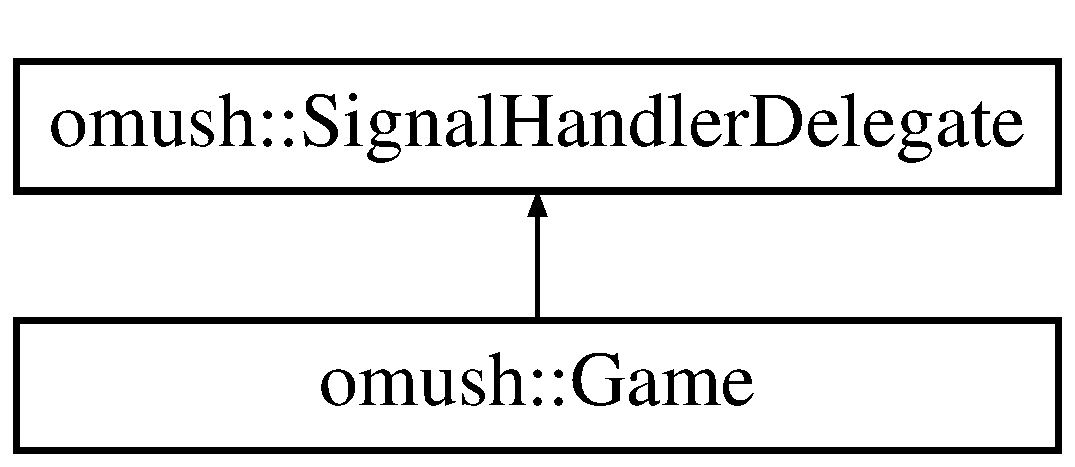
\includegraphics[height=2.000000cm]{classomush_1_1_game}
\end{center}
\end{figure}
\subsection*{Public Member Functions}
\begin{DoxyCompactItemize}
\item 
\hyperlink{classomush_1_1_game_a6e4e5e9f6edf99893895d0261423afc1}{Game} ()
\item 
\hyperlink{classomush_1_1_game_a8dd181346e8a62be54585a20b5e52588}{$\sim$\-Game} ()
\item 
void \hyperlink{classomush_1_1_game_aae6eb03bcbc479ce68eaf6a1b449665a}{run} ()
\item 
virtual void \hyperlink{classomush_1_1_game_a90582895228ea196287a36d35d21f3ba}{handle\-Signal} (int signal)
\end{DoxyCompactItemize}


\subsection{Detailed Description}
This is the main class that is the the game. Everything is handled from here. 

\subsection{Constructor \& Destructor Documentation}
\hypertarget{classomush_1_1_game_a6e4e5e9f6edf99893895d0261423afc1}{\index{omush\-::\-Game@{omush\-::\-Game}!Game@{Game}}
\index{Game@{Game}!omush::Game@{omush\-::\-Game}}
\subsubsection[{Game}]{\setlength{\rightskip}{0pt plus 5cm}omush\-::\-Game\-::\-Game (
\begin{DoxyParamCaption}
{}
\end{DoxyParamCaption}
)}}\label{classomush_1_1_game_a6e4e5e9f6edf99893895d0261423afc1}
Constructor. Do any initial resetting or setup of theg game that doesn't require on external configuration. \hypertarget{classomush_1_1_game_a8dd181346e8a62be54585a20b5e52588}{\index{omush\-::\-Game@{omush\-::\-Game}!$\sim$\-Game@{$\sim$\-Game}}
\index{$\sim$\-Game@{$\sim$\-Game}!omush::Game@{omush\-::\-Game}}
\subsubsection[{$\sim$\-Game}]{\setlength{\rightskip}{0pt plus 5cm}omush\-::\-Game\-::$\sim$\-Game (
\begin{DoxyParamCaption}
{}
\end{DoxyParamCaption}
)}}\label{classomush_1_1_game_a8dd181346e8a62be54585a20b5e52588}
Destructor. Free up any resources that were allocated during the lifetime of the game. 

\subsection{Member Function Documentation}
\hypertarget{classomush_1_1_game_a90582895228ea196287a36d35d21f3ba}{\index{omush\-::\-Game@{omush\-::\-Game}!handle\-Signal@{handle\-Signal}}
\index{handle\-Signal@{handle\-Signal}!omush::Game@{omush\-::\-Game}}
\subsubsection[{handle\-Signal}]{\setlength{\rightskip}{0pt plus 5cm}void omush\-::\-Game\-::handle\-Signal (
\begin{DoxyParamCaption}
\item[{int}]{signum}
\end{DoxyParamCaption}
)\hspace{0.3cm}{\ttfamily [virtual]}}}\label{classomush_1_1_game_a90582895228ea196287a36d35d21f3ba}
Handle S\-I\-G\-I\-N\-T by setting the shutdown flag on the game.


\begin{DoxyParams}{Parameters}
{\em signum} & Signal caught by \hyperlink{classomush_1_1_signal_handler}{Signal\-Handler}. \\
\hline
\end{DoxyParams}


Implements \hyperlink{classomush_1_1_signal_handler_delegate}{omush\-::\-Signal\-Handler\-Delegate}.

\hypertarget{classomush_1_1_game_aae6eb03bcbc479ce68eaf6a1b449665a}{\index{omush\-::\-Game@{omush\-::\-Game}!run@{run}}
\index{run@{run}!omush::Game@{omush\-::\-Game}}
\subsubsection[{run}]{\setlength{\rightskip}{0pt plus 5cm}void omush\-::\-Game\-::run (
\begin{DoxyParamCaption}
{}
\end{DoxyParamCaption}
)}}\label{classomush_1_1_game_aae6eb03bcbc479ce68eaf6a1b449665a}
The main loop of the program. When this method returns, the program should end. 

The documentation for this class was generated from the following files\-:\begin{DoxyCompactItemize}
\item 
omush/hdrs/omush/game.\-h\item 
omush/src/game.\-cc\end{DoxyCompactItemize}

\hypertarget{classomush_1_1_signal_handler}{\section{omush\-:\-:Signal\-Handler Class Reference}
\label{classomush_1_1_signal_handler}\index{omush\-::\-Signal\-Handler@{omush\-::\-Signal\-Handler}}
}


{\ttfamily \#include $<$signalhandler.\-h$>$}

\subsection*{Static Public Member Functions}
\begin{DoxyCompactItemize}
\item 
static void \hyperlink{classomush_1_1_signal_handler_af5c48427c63f6b41ce3436d585607377}{register\-Delegate} (\hyperlink{classomush_1_1_signal_handler_delegate}{Signal\-Handler\-Delegate} $\ast$, int)
\item 
static void \hyperlink{classomush_1_1_signal_handler_aa0dbf3364fde042272f2ca76abaed61e}{setup\-Signal\-Handling} ()
\item 
static void \hyperlink{classomush_1_1_signal_handler_ae80806a7f8ab6fdbd57740eab52d401e}{signal\-Handler} (int signum)
\end{DoxyCompactItemize}


\subsection{Detailed Description}
Static class that handles catching signals. 

\subsection{Member Function Documentation}
\hypertarget{classomush_1_1_signal_handler_af5c48427c63f6b41ce3436d585607377}{\index{omush\-::\-Signal\-Handler@{omush\-::\-Signal\-Handler}!register\-Delegate@{register\-Delegate}}
\index{register\-Delegate@{register\-Delegate}!omush::SignalHandler@{omush\-::\-Signal\-Handler}}
\subsubsection[{register\-Delegate}]{\setlength{\rightskip}{0pt plus 5cm}void omush\-::\-Signal\-Handler\-::register\-Delegate (
\begin{DoxyParamCaption}
\item[{{\bf Signal\-Handler\-Delegate} $\ast$}]{delegate, }
\item[{int}]{signal}
\end{DoxyParamCaption}
)\hspace{0.3cm}{\ttfamily [static]}}}\label{classomush_1_1_signal_handler_af5c48427c63f6b41ce3436d585607377}
Register an instance of \hyperlink{classomush_1_1_signal_handler_delegate}{Signal\-Handler\-Delegate} to receive siginals.


\begin{DoxyParams}{Parameters}
{\em delegate} & Instance of Siginal\-Handler\-Delegate that will receive the signal. \\
\hline
{\em signal} & The signal that the delegate will respond to. \\
\hline
\end{DoxyParams}
\hypertarget{classomush_1_1_signal_handler_aa0dbf3364fde042272f2ca76abaed61e}{\index{omush\-::\-Signal\-Handler@{omush\-::\-Signal\-Handler}!setup\-Signal\-Handling@{setup\-Signal\-Handling}}
\index{setup\-Signal\-Handling@{setup\-Signal\-Handling}!omush::SignalHandler@{omush\-::\-Signal\-Handler}}
\subsubsection[{setup\-Signal\-Handling}]{\setlength{\rightskip}{0pt plus 5cm}void omush\-::\-Signal\-Handler\-::setup\-Signal\-Handling (
\begin{DoxyParamCaption}
{}
\end{DoxyParamCaption}
)\hspace{0.3cm}{\ttfamily [static]}}}\label{classomush_1_1_signal_handler_aa0dbf3364fde042272f2ca76abaed61e}
Register any siginals we care about in the application. Those siginals will be caught by \hyperlink{classomush_1_1_signal_handler_ae80806a7f8ab6fdbd57740eab52d401e}{signal\-Handler()}. \hypertarget{classomush_1_1_signal_handler_ae80806a7f8ab6fdbd57740eab52d401e}{\index{omush\-::\-Signal\-Handler@{omush\-::\-Signal\-Handler}!signal\-Handler@{signal\-Handler}}
\index{signal\-Handler@{signal\-Handler}!omush::SignalHandler@{omush\-::\-Signal\-Handler}}
\subsubsection[{signal\-Handler}]{\setlength{\rightskip}{0pt plus 5cm}void omush\-::\-Signal\-Handler\-::signal\-Handler (
\begin{DoxyParamCaption}
\item[{int}]{signum}
\end{DoxyParamCaption}
)\hspace{0.3cm}{\ttfamily [static]}}}\label{classomush_1_1_signal_handler_ae80806a7f8ab6fdbd57740eab52d401e}
Method to intercept singals. Registered by setup\-Siginal\-Handling().

Will call handle\-Signal() on any \hyperlink{classomush_1_1_signal_handler_delegate}{Signal\-Handler\-Delegate} that has registered with signum. Signum is passed to handle\-Signal() so the \hyperlink{classomush_1_1_signal_handler_delegate}{Signal\-Handler\-Delegate} knows how to handle it.


\begin{DoxyParams}{Parameters}
{\em signum} & The siginal caught by the class. \\
\hline
\end{DoxyParams}


The documentation for this class was generated from the following files\-:\begin{DoxyCompactItemize}
\item 
omush/hdrs/omush/signalhandler.\-h\item 
omush/src/signalhandler.\-cc\end{DoxyCompactItemize}

\hypertarget{classomush_1_1_signal_handler_delegate}{\section{omush\-:\-:Signal\-Handler\-Delegate Class Reference}
\label{classomush_1_1_signal_handler_delegate}\index{omush\-::\-Signal\-Handler\-Delegate@{omush\-::\-Signal\-Handler\-Delegate}}
}


{\ttfamily \#include $<$signalhandler.\-h$>$}

Inheritance diagram for omush\-:\-:Signal\-Handler\-Delegate\-:\begin{figure}[H]
\begin{center}
\leavevmode
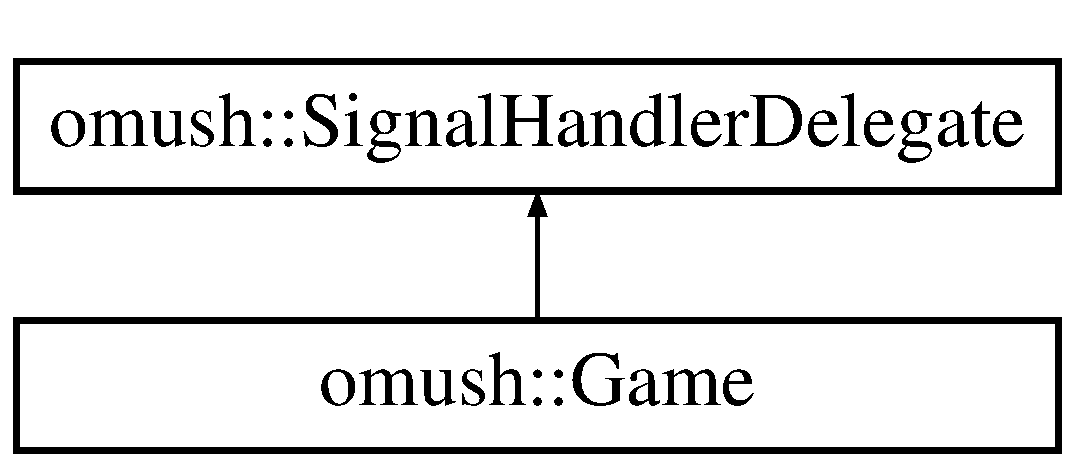
\includegraphics[height=2.000000cm]{classomush_1_1_signal_handler_delegate}
\end{center}
\end{figure}
\subsection*{Public Member Functions}
\begin{DoxyCompactItemize}
\item 
\hypertarget{classomush_1_1_signal_handler_delegate_a8900e60d39bbc2c62b69b5aa74bd5c04}{virtual void {\bfseries handle\-Signal} (int signal)=0}\label{classomush_1_1_signal_handler_delegate_a8900e60d39bbc2c62b69b5aa74bd5c04}

\end{DoxyCompactItemize}


\subsection{Detailed Description}
Delegatge interface for any object that needs to handle signals. 

The documentation for this class was generated from the following file\-:\begin{DoxyCompactItemize}
\item 
omush/hdrs/omush/signalhandler.\-h\end{DoxyCompactItemize}

%--- End generated contents ---

% Index
\newpage
\phantomsection
\addcontentsline{toc}{chapter}{Index}
\printindex

\end{document}
